% Optional LaTeX snippets for the generated baseline figures.
% Paths are relative to the repository root.

\begin{figure}[t]
  \centering
  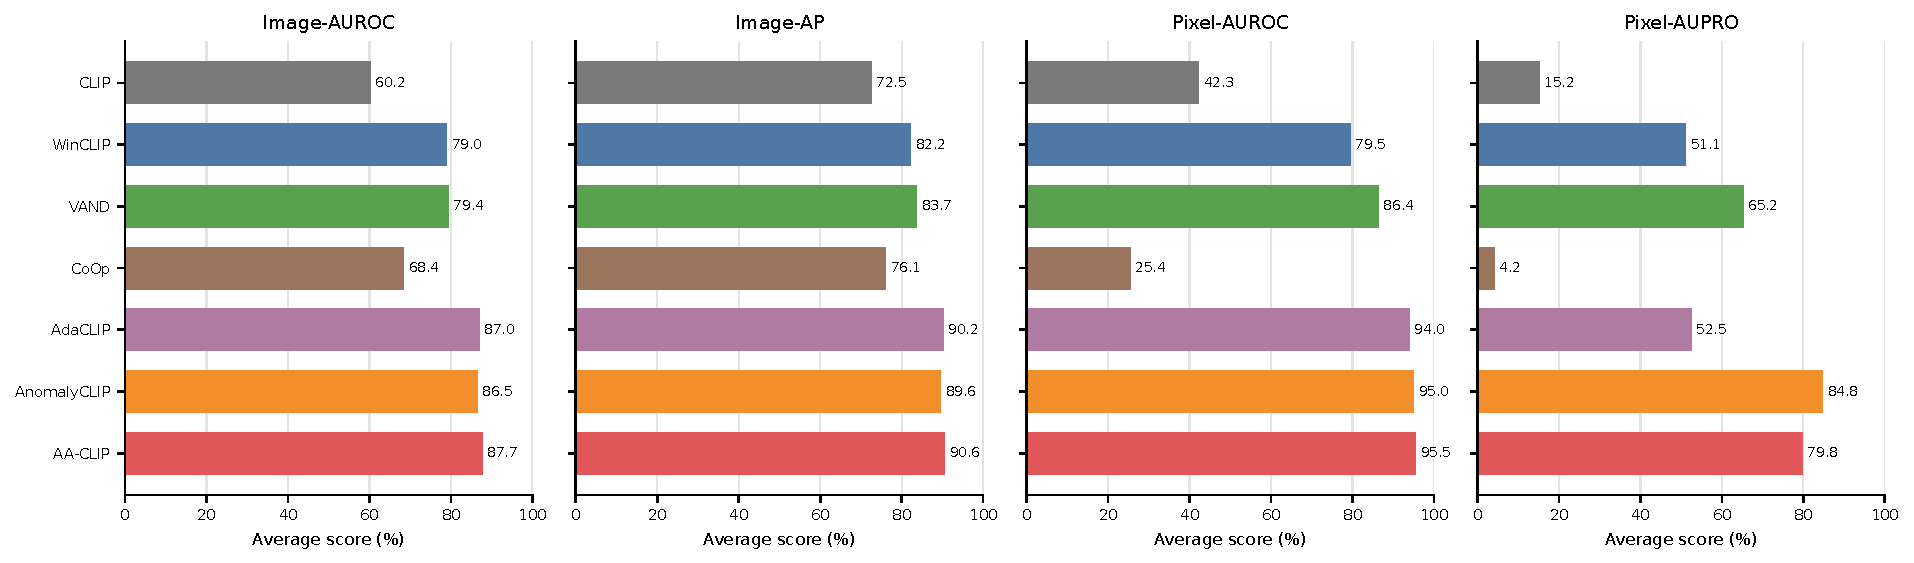
\includegraphics[width=0.98\textwidth]{paper/figures_iconip_baselines/figures/industrial_average_baseline_bars.pdf}
  \caption{Average baseline performance on industrial anomaly detection benchmarks.}
  \label{fig:industrial_baseline_average_bars}
\end{figure}

\begin{figure}[t]
  \centering
  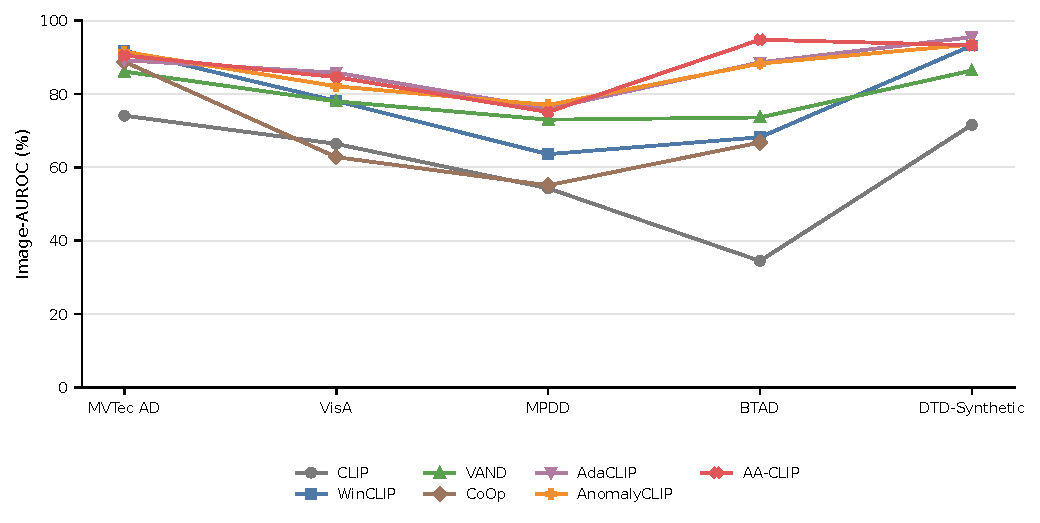
\includegraphics[width=0.98\textwidth]{paper/figures_iconip_baselines/figures/industrial_image_auroc_baseline_lines.pdf}
  \caption{Industrial image-level AUROC baseline comparison across datasets.}
  \label{fig:industrial_image_auroc_baseline_lines}
\end{figure}

\begin{figure}[t]
  \centering
  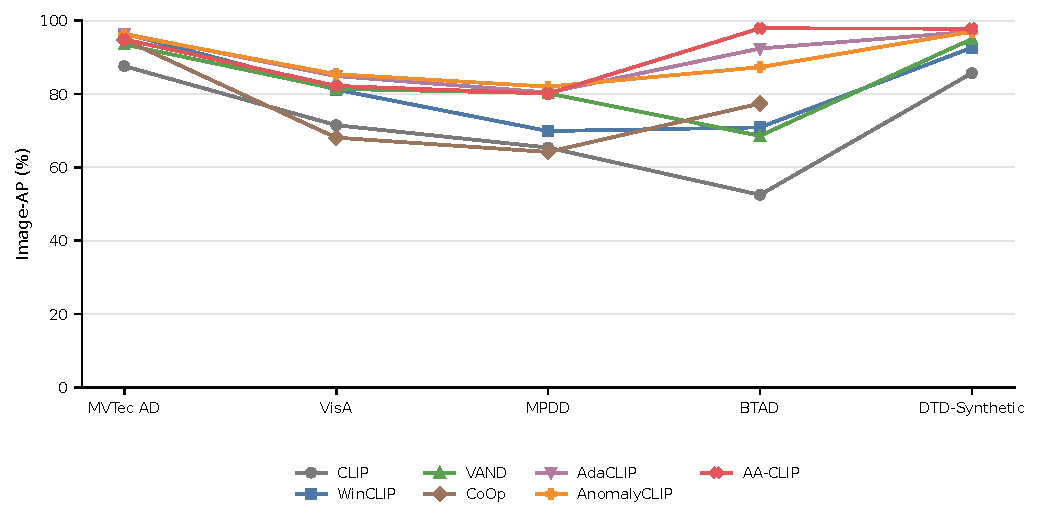
\includegraphics[width=0.98\textwidth]{paper/figures_iconip_baselines/figures/industrial_image_ap_baseline_lines.pdf}
  \caption{Industrial image-level AP baseline comparison across datasets.}
  \label{fig:industrial_image_ap_baseline_lines}
\end{figure}

\begin{figure}[t]
  \centering
  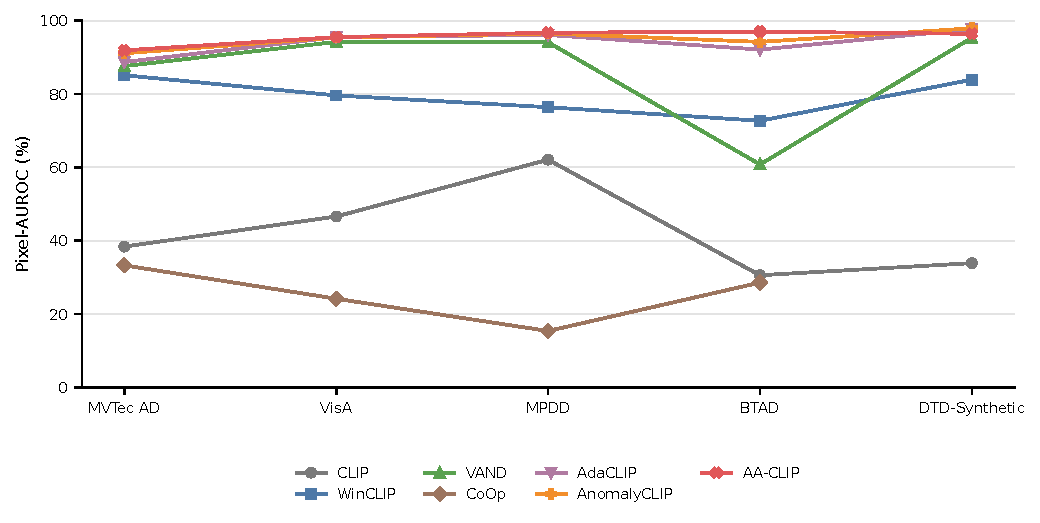
\includegraphics[width=0.98\textwidth]{paper/figures_iconip_baselines/figures/industrial_pixel_auroc_baseline_lines.pdf}
  \caption{Industrial pixel-level AUROC baseline comparison across datasets.}
  \label{fig:industrial_pixel_auroc_baseline_lines}
\end{figure}

\begin{figure}[t]
  \centering
  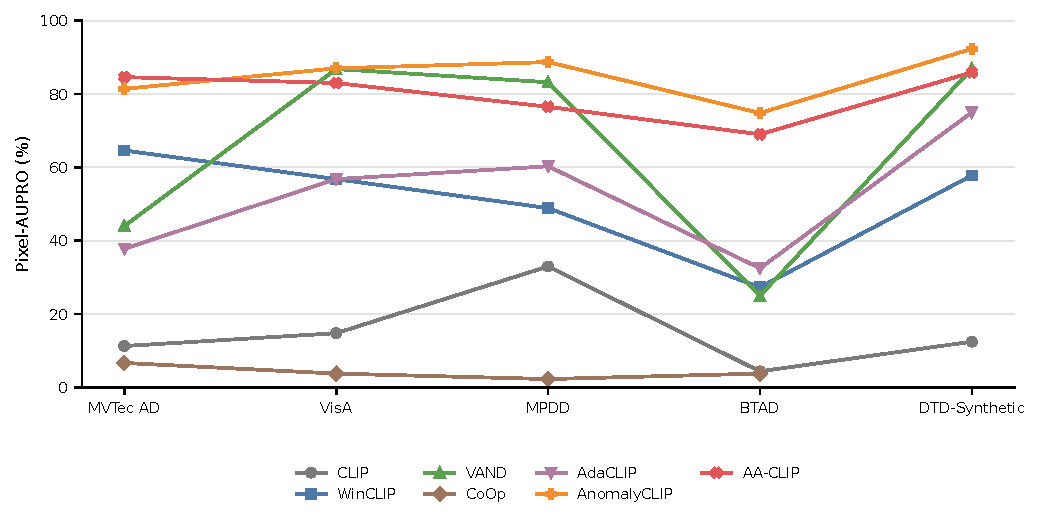
\includegraphics[width=0.98\textwidth]{paper/figures_iconip_baselines/figures/industrial_pixel_aupro_baseline_lines.pdf}
  \caption{Industrial pixel-level AUPRO baseline comparison across datasets.}
  \label{fig:industrial_pixel_aupro_baseline_lines}
\end{figure}

\begin{figure}[t]
  \centering
  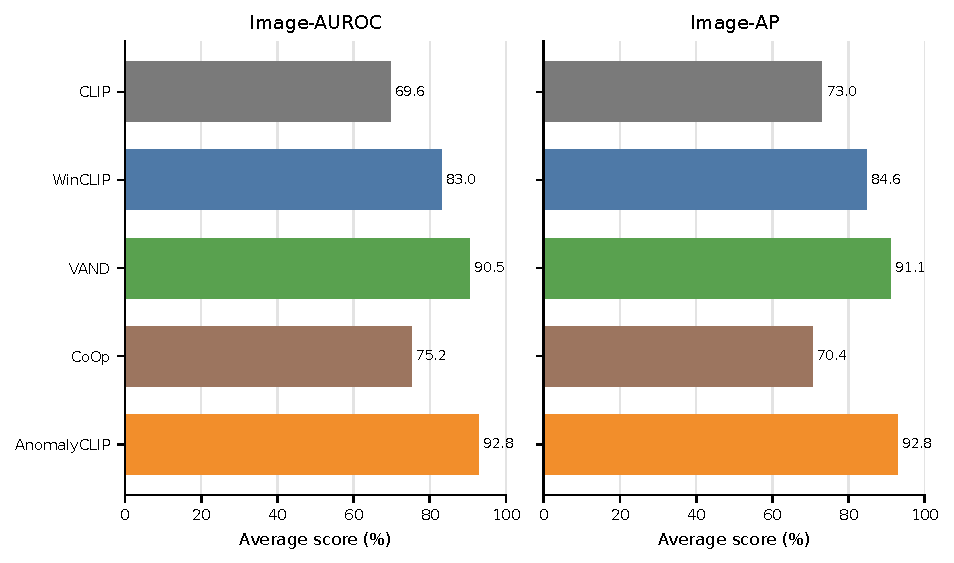
\includegraphics[width=0.78\textwidth]{paper/figures_iconip_baselines/figures/medical_image_average_baseline_bars.pdf}
  \caption{Average image-level baseline performance on medical anomaly detection benchmarks.}
  \label{fig:medical_image_baseline_average_bars}
\end{figure}

\begin{figure}[t]
  \centering
  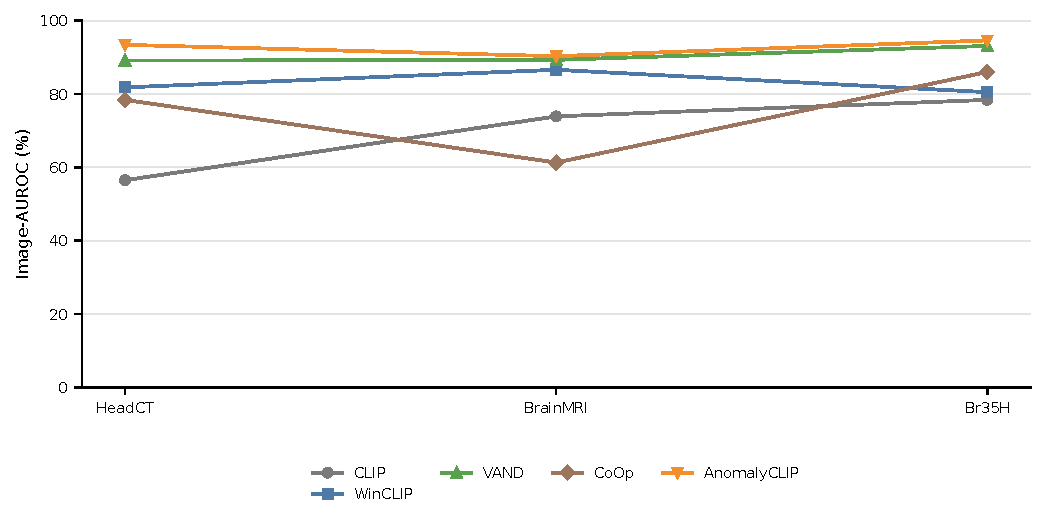
\includegraphics[width=0.78\textwidth]{paper/figures_iconip_baselines/figures/medical_image_auroc_baseline_lines.pdf}
  \caption{Medical image-level AUROC baseline comparison across datasets.}
  \label{fig:medical_image_auroc_baseline_lines}
\end{figure}

\begin{figure}[t]
  \centering
  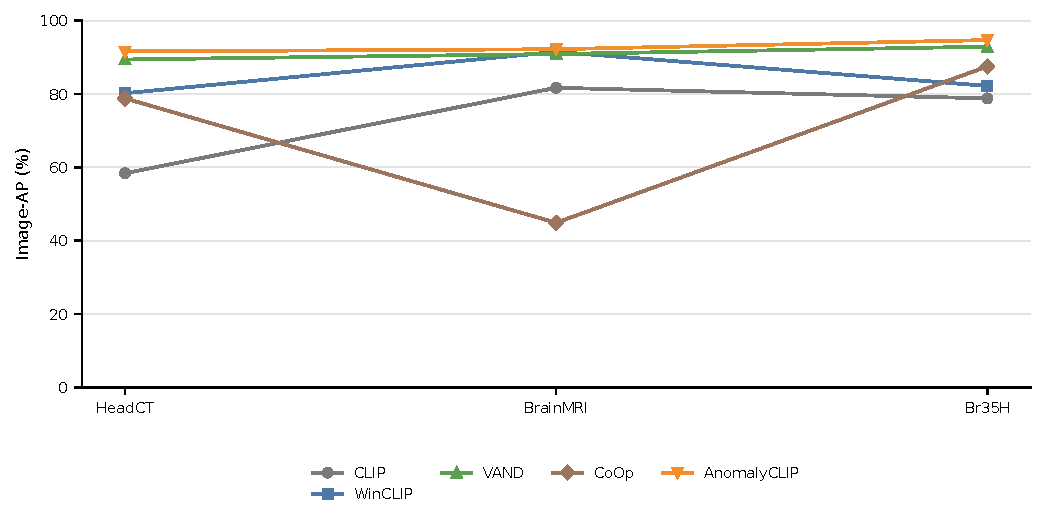
\includegraphics[width=0.78\textwidth]{paper/figures_iconip_baselines/figures/medical_image_ap_baseline_lines.pdf}
  \caption{Medical image-level AP baseline comparison across datasets.}
  \label{fig:medical_image_ap_baseline_lines}
\end{figure}

\begin{figure}[t]
  \centering
  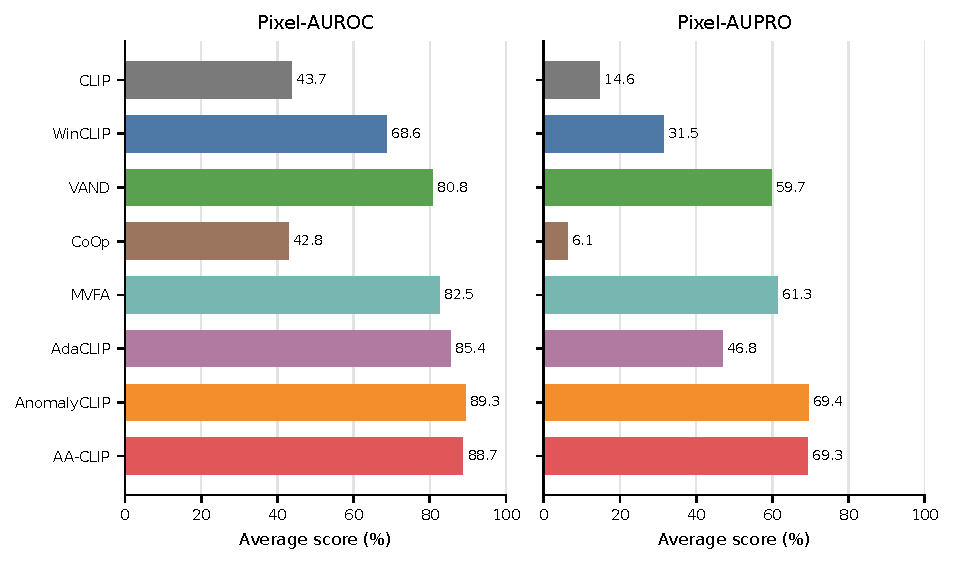
\includegraphics[width=0.78\textwidth]{paper/figures_iconip_baselines/figures/medical_pixel_average_baseline_bars.pdf}
  \caption{Average pixel-level baseline performance on medical anomaly localization benchmarks.}
  \label{fig:medical_pixel_baseline_average_bars}
\end{figure}

\begin{figure}[t]
  \centering
  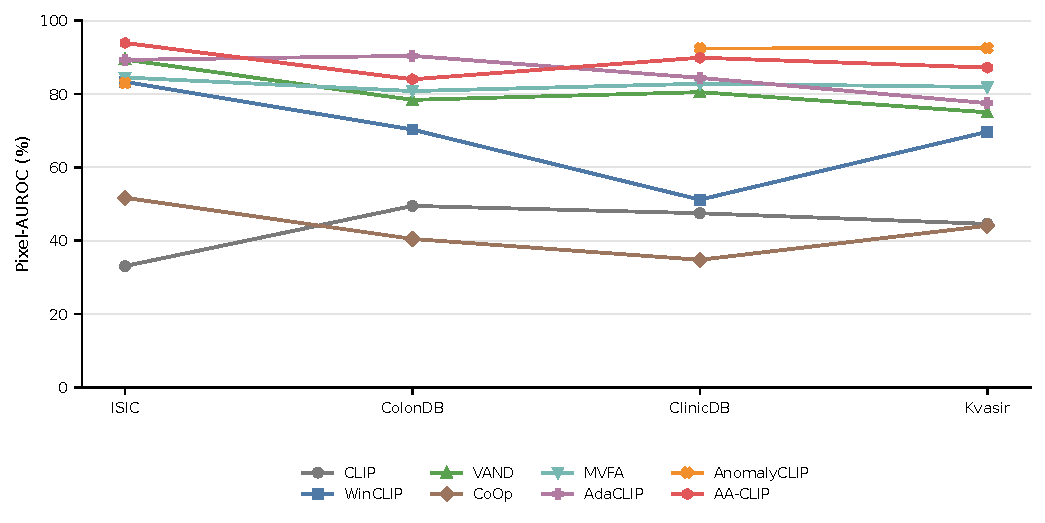
\includegraphics[width=0.98\textwidth]{paper/figures_iconip_baselines/figures/medical_pixel_auroc_baseline_lines.pdf}
  \caption{Medical pixel-level AUROC baseline comparison across datasets.}
  \label{fig:medical_pixel_auroc_baseline_lines}
\end{figure}

\begin{figure}[t]
  \centering
  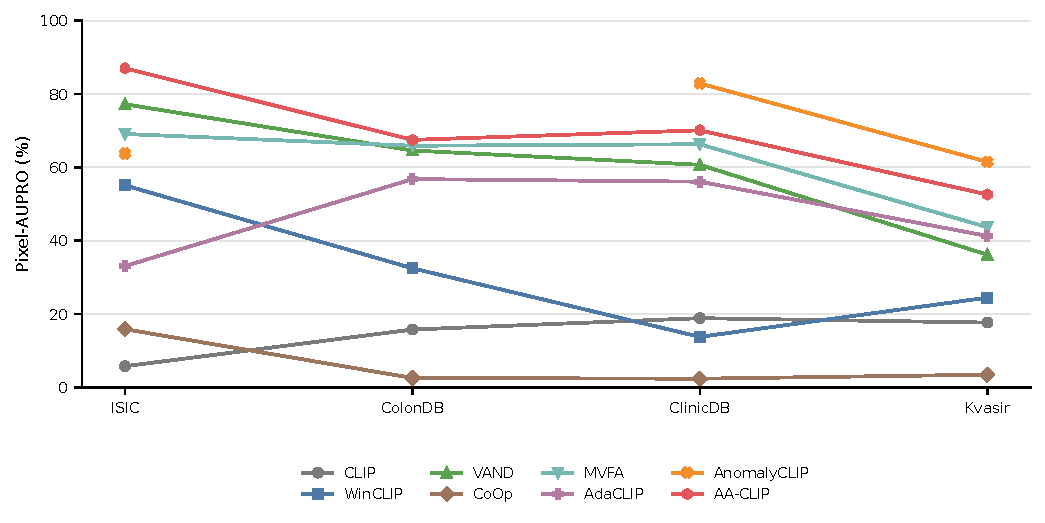
\includegraphics[width=0.98\textwidth]{paper/figures_iconip_baselines/figures/medical_pixel_aupro_baseline_lines.pdf}
  \caption{Medical pixel-level AUPRO baseline comparison across datasets.}
  \label{fig:medical_pixel_aupro_baseline_lines}
\end{figure}
